\documentclass{article}
\usepackage{graphicx, amsmath, subcaption} % Required for inserting images

\title{Comparative Analysis of Algorithms on CEC 2017 Benchmarks}
% \subtitle{SDSC3004 Final Project Report}
\author{Yue ZHU}
% \institute{City University of Hong Kong}
\date{April 2026}

\begin{document}

\maketitle

\section{Introduction}

This project focuses on the Comparative Analysis of Algorithms which tested on selected CEC 2017 benchmarks. Four benchmarks from four different types of problems were chosen, which are Unimodal (No.2), Multimodal (No.10), Hybrid (No.17), and Composition (No.27). 

For the algorithms, we chose 3 families of algorithms, which consists of 3 basic algorithms, \textbf{Differential Evolution (DE)}, \textbf{Simulated Annealing (SA)}, and \textbf{Spherical Search (SS)}, and 3 upgraded algorithms, \textbf{Self-Adapted Differential Evolution (jDE)}, \textbf{Dual Annealing (DA)}, and \textbf{Self-Adapted Spherical Search (SASS)}.

\section{Methodology}

To compare these 6 algorithms strictly and fairly, we designed a completed experimental setting and apply to every experiments. 

\subsection{Experimental Settings}

To ensure absolute statistical rigor, all algorithms were subjected to the exact same constraints:

\begin{itemize}
    \item \textbf{Dimensionality:} $D = 30$ for all problems, with search bounds $(-100, 100)$.
    \item \textbf{Statistical Robustness:} 10 independent runs per algorithm to account for stochastic variance. Results report the Mean and Min/Max margins.
    \item \textbf{The Metric of Fairness:} Function Evaluations (FEs). In the experiments, we set the maximum function evaluations as 300,000.
\end{itemize}

\section{Algorithm Overview}

\subsection*{Differential Evolution Family}

\textbf{Differential Evolution (DE)} is a population-based optimization algorithm. It evolves a population using vector mathematics, specifically updating positions based on the physical distance between members to naturally scale search steps. DE will initialize a population of candidate solutions based on pop\_size, and iteratively apply mutation and crossover operations to evolve the population towards optimal solutions. The core formula for mutation is:

\[v_{i} = x_{r1} + F \cdot (x_{r2} - x_{r3})\]
where $v_i$ is the mutant vector, $x_{r1}$, $x_{r2}$, and $x_{r3}$ are randomly selected individuals from the population, and $F$ is the mutation scaling factor. The crossover operation then combines the mutant vector with the current individual to create a trial vector, which is evaluated and potentially replaces the current individual based on fitness.

\textbf{Self-Adapted Differential Evolution (jDE)} is an enhanced version of DE that incorporates self-adaptation mechanisms for its control parameters. In jDE, the mutation scaling factor $F$ and crossover rate $C$ are not fixed but evolve alongside the population. Each individual in the population has its own $F$ and $C$ values, which are updated based on their performance. The algorithm includes a trial mechanism where, with a trial probability (trial\_prob), new random values for $F$ and $C$ are generated, allowing the algorithm to dynamically adjust its search strategy over time.

\subsection*{Simulated Annealing Family}

\textbf{Simulated Annealing (SA)} is a single-solution based optimization algorithm inspired by the annealing process in metallurgy. It starts with an initial solution and iteratively explores the solution space by making random perturbations. The acceptance of new solutions is governed by a probability that depends on the change in objective function value and a temperature parameter. The algorithm allows for occasional acceptance of worse solutions to escape local minima, with the probability of 
\[\exp\left(\frac{\Delta E}{T_k}\right)\]
where $\Delta E$ is the change in the objective function value and $T_k$ is the current temperature. As the algorithm progresses, the temperature is gradually reduced according to a cooling schedule. The cooling schedule is typically defined as:
\[T_{k+1} = T_k \cdot \text{cooling\_rate}\]
where $T_k$ is the temperature at iteration $k$.

\textbf{Dual Annealing (DA)} is an advanced variant of simulated annealing that combines the principles of both global and local search. It utilizes a dual approach where the algorithm alternates between a global search phase, which explores the solution space broadly, and a local search phase, which focuses on refining promising solutions. DA incorporates a more sophisticated cooling schedule and acceptance criteria, allowing it to effectively navigate complex optimization landscapes. The algorithm is designed to balance exploration and exploitation, making it particularly effective for high-dimensional and multimodal optimization problems.

\subsection*{Spherical Search Family}

\textbf{Spherical Search (SS)} is also a population-based optimization algorithm, but it operates on a spherical coordinate system, instead of the standard Cartesian system. The algorithm generates new candidate solutions by perturbing the current population in a spherical manner, which allows for more diverse search patterns. The mutation operation in SS is defined as:
\[v_{i} = x_{i} + c \cdot \text{randn}(0, 1) \cdot \frac{(x_{r1} - x_{r2})}{\|x_{r1} - x_{r2}\|}\]
where $v_i$ is the mutant vector, $x_i$ is the current individual, $c$ is a fixed mutation factor, $\text{randn}(0, 1)$ is a random number drawn from a standard normal distribution, and $x_{r1}$ and $x_{r2}$ are randomly selected individuals from the population. The crossover operation in SS is similar to that of DE, where a trial vector is created by combining the mutant vector with the current individual based on a fixed crossover rate.

\textbf{Self-Adapted Spherical Search (SASS)} is an enhanced version of the Spherical Search algorithm that incorporates self-adaptation mechanisms for its control parameters. In SASS, the mutation factor $c$ and crossover rate $rp$ are not fixed but evolve alongside the population. Each individual in the population has its own $c$ and $rp$ values, which are updated based on their performance. The mutation factors are generated from a standard Cauchy distribution, while the crossover rates are generated from a standard normal distribution. This self-adaptation allows SASS to dynamically adjust its search strategy over time, improving its ability to navigate complex optimization landscapes.

\subsection{Algorithm Running Settings}

\subsubsection*{Differential Evolution}

\begin{itemize}
    \item pop\_size = 100 (Population Size)
    \item F = 0.5 (Mutation Scaling Factor)
    \item C = 0.9 (Crossover Rate)
\end{itemize}

\subsubsection*{Self-Adapted Differential Evolution}

\begin{itemize}
    \item pop\_size = 100 (Population Size)
    \item F\_array = $[0.5, \ldots, 0.5]$ (Initial Mutation Scaling Factor Array)
    \item C\_array = $[0.9, \ldots, 0.9]$ (Initial Crossover Rate)
    \item trial\_prob = 0.1 (Probability of Taking a Random Trial of F and C)
\end{itemize}

\subsubsection*{Simulated Annealing}

\begin{itemize}
    \item initial\_temp = 10000 (Initial Temperature)
    \item cooling\_rate = 0.99999 (Cooling Rate, ending temperature at 497.86)
    \item noise = np.random.normal(loc=0, scale=5.0, size=dim) (Noise sampled from $N(\mu=0, \sigma=5.0)$)
\end{itemize}

\subsubsection*{Dual Annealing}

\begin{itemize}
    \item initial\_temp = 5230 (Initial Temperature)
    \item Function called from scipy.optimize
\end{itemize}

\subsubsection*{Spherical Search}

\begin{itemize}
    \item pop\_size = 150 (Population Size)
    \item c = 0.8 (Fixed Mutation Factor)
    \item rp = 0.5 (Fixed Crossover Rate)
\end{itemize}

\subsubsection*{Self-Adapted Spherical Search}

\begin{itemize}
    \item pop\_size = 150 (Population Size)
    \item memory\_size = 5 (Parameter History Storage Size)
    \item Mutation Factors were generated from Standard Cauchy Distribution
    \item Crossover Rate were generated from Standard Normal Distribution
\end{itemize}

\section{Results and Analysis}

The results of the experiments are summarized in the following table, which reports the mean and minimum values of the objective function for each algorithm across the 10 independent runs on each benchmark problem.

\noindent\resizebox{\textwidth}{!}{
        \begin{tabular}{|l||c|c|c|c|}
        \hline
        \textbf{Algorithm} & \textbf{Unimodal (NO2)} & \textbf{Multimodal (NO10)} & \textbf{Hybrid (NO17)} & \textbf{Composition (NO27)} \\ \hline \hline
        
        \textbf{Global Optimum} & \textbf{200.00} & \textbf{1000.00} & \textbf{1700.00} & \textbf{2700.00} \\ \hline \hline

        \textbf{DE}        & 2336.4 / (464.8)   & 52577.2 / (16910.5)   & 2091.7 / (59.1)    & 3178.7 / (295.1)    \\ \hline
        \textbf{jDE}       & \textbf{200.00 / (0.0)}      & 1241.6 / (25.8)     & 1927.8 / (34.7)    & \textbf{2707.2 / (0.0)}      \\ \hline
        \textbf{SA}        & 6895.6 / (5468.4)     & 193251.2 / (108318.3)   & 210818.4 / (133176.8) & 6528.3 / (2135.1)     \\ \hline
        \textbf{DA}        & \textbf{200.00 / (0.0)}      & 1546.5 / (212.9)     & \textbf{1742.9 / (31.1)}    & \textbf{2766.1 / (24.6)}      \\ \hline
        \textbf{SS}        & \textbf{200.00 / (0.0)}      & 121738.5 / (30673.7)   & 419256.3 / (242213.8) & \textbf{2700.0 / (0.0)}      \\ \hline
        \textbf{SASS}      & \textbf{200.00 / (0.0)} & \textbf{1017.7 / (6.9)} & \textbf{1722.1 / (20.1)} & \textbf{2716.9 / (0.0)} \\ \hline
        
        \end{tabular}
    }
\vspace{0.5cm}

From the table, we can observe that the upgraded algorithms (jDE, DA, and SASS) generally outperform their basic counterparts (DE, SA, and SS) across all benchmark problems. Notably, jDE, DA, and Spherical Search Family achieved the global optimum on the Unimodal problem (No.2). The Composition problem (No.27) saw strong performance from jDE, DA, SS, and SASS, with all four algorithms achieving optimal or near-optimal results. However, the Multimodal (No.10) and Hybrid (No.17) problems presented more challenges, with only SASS achieving the near-optimum on both, while only DA achieved the near-optimum on the Hybrid problem (No.17). The basic algorithms, particularly SA and SS, struggled significantly on the Multimodal and Hybrid problems, indicating their limitations in navigating complex search spaces.

\begin{figure}[htbp]
     \centering
     % Row 1
     \begin{subfigure}{0.49\textwidth}
         \centering
         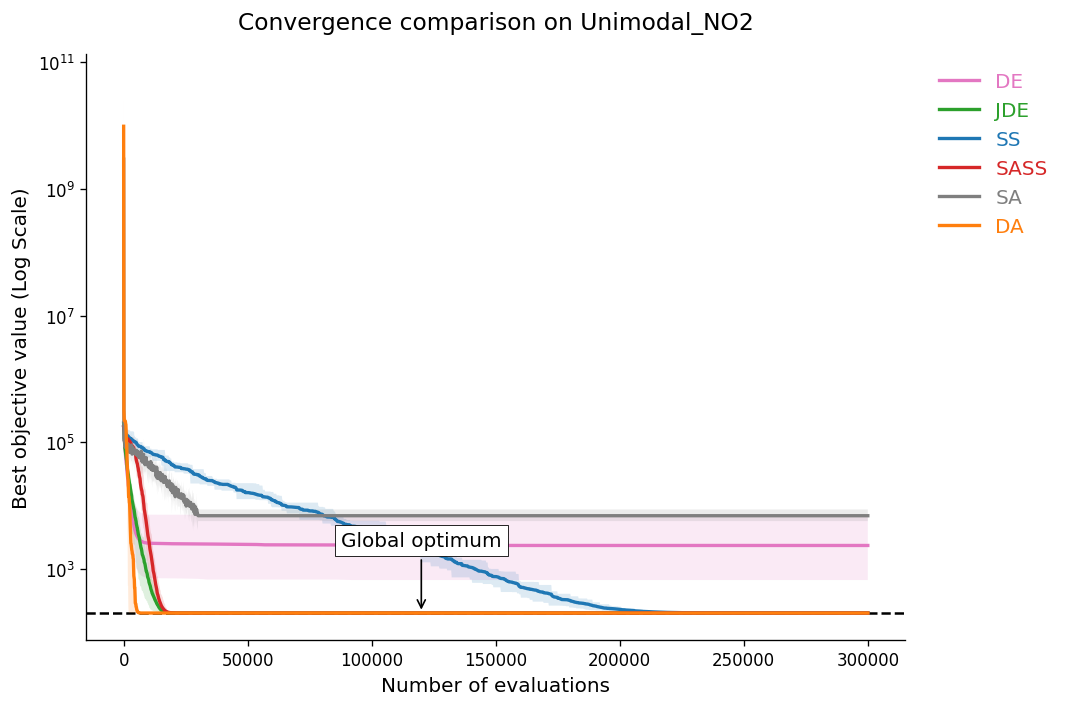
\includegraphics[width=\textwidth]{no2_conv.png}
         \label{fig:image1}
     \end{subfigure}
     \hfill
     \begin{subfigure}{0.49\textwidth}
         \centering
         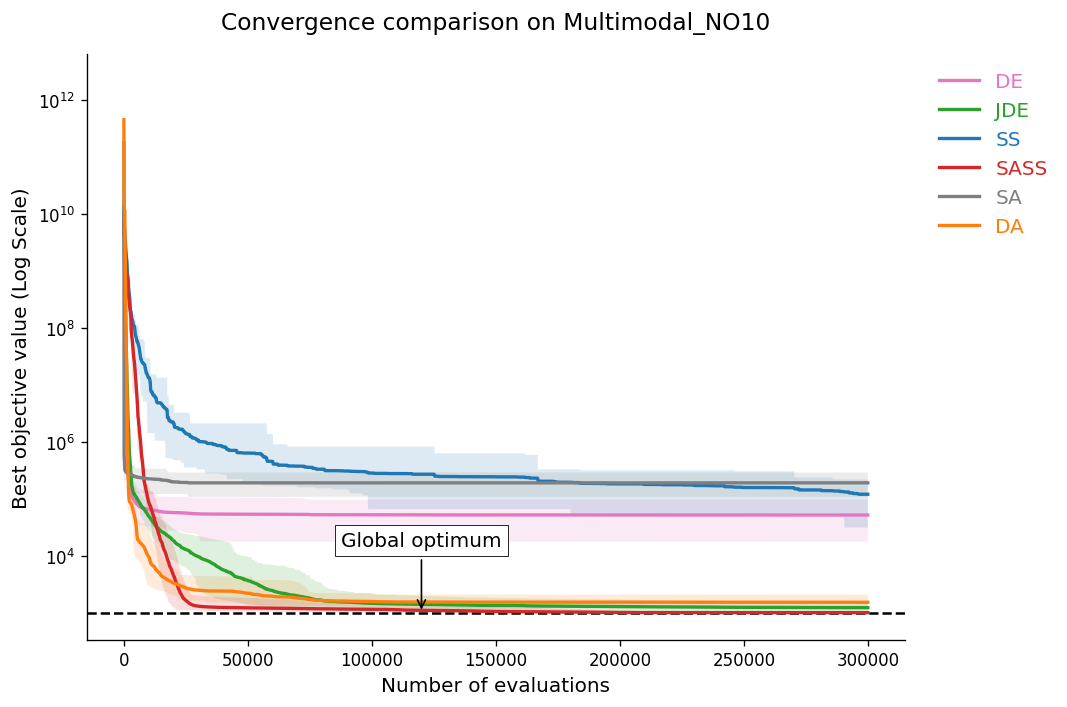
\includegraphics[width=\textwidth]{no10_conv.png}
         \label{fig:image2}
     \end{subfigure}

     \vspace{0.05cm} % Adjust vertical gap between rows

     % Row 2
     \begin{subfigure}{0.49\textwidth}
         \centering
         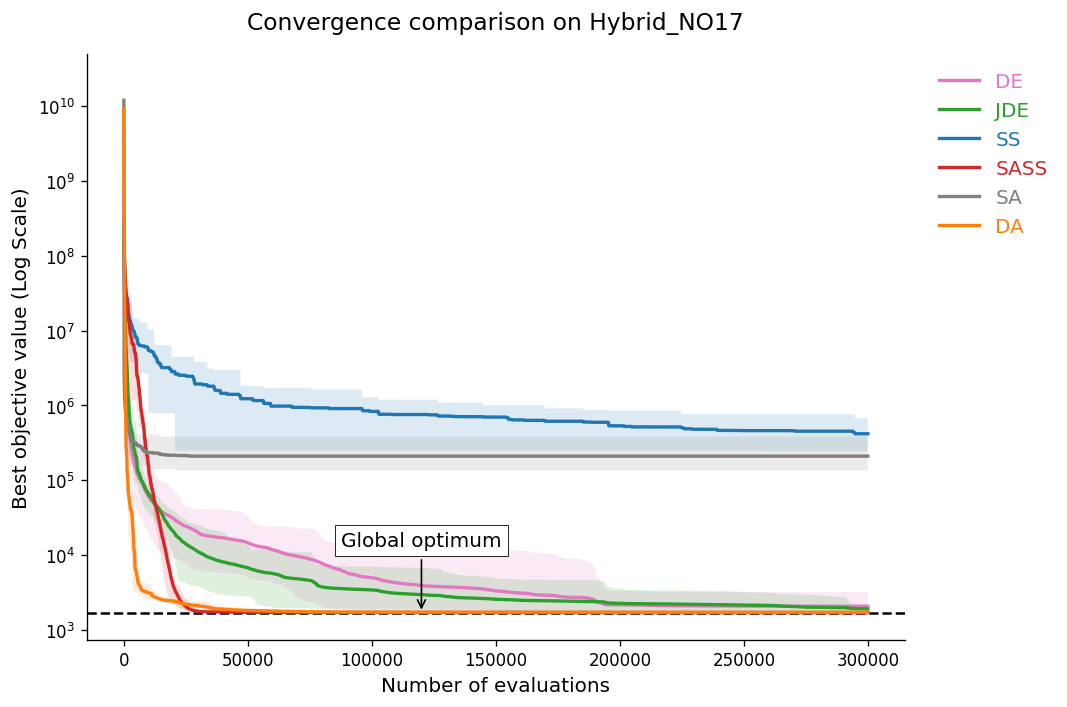
\includegraphics[width=\textwidth]{no17_conv.png}
         \label{fig:image3}
     \end{subfigure}
     \hfill
     \begin{subfigure}{0.49\textwidth}
         \centering
         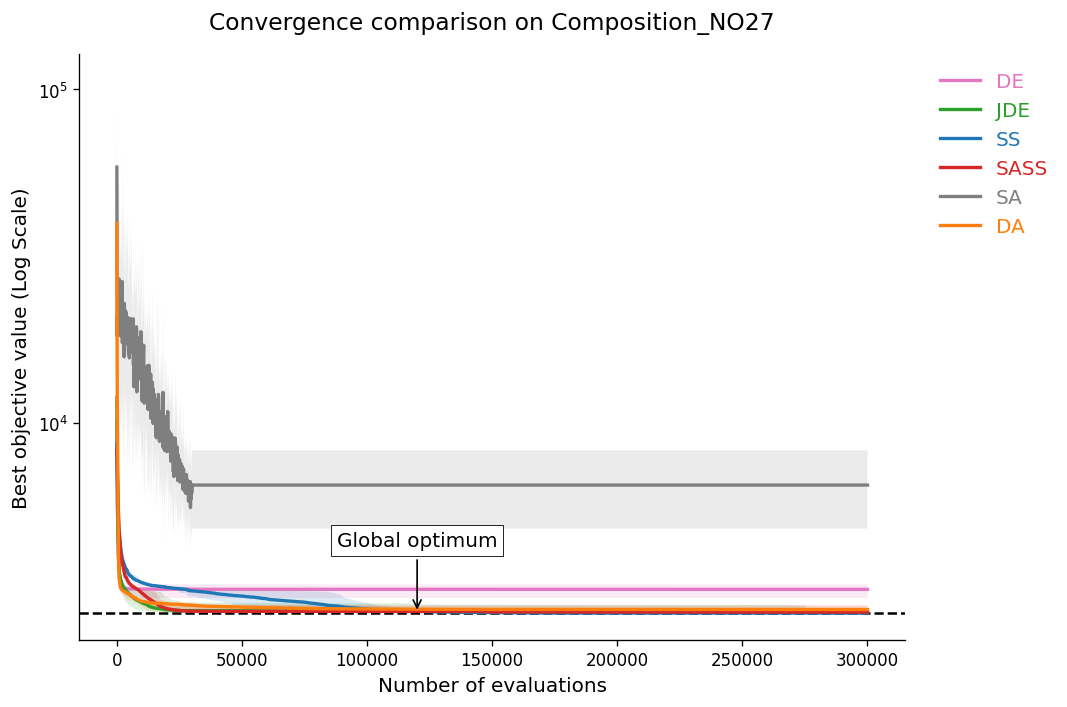
\includegraphics[width=\textwidth]{no27_conv.png}
         \label{fig:image4}
     \end{subfigure}
     
    %  \vspace{0.3cm}
     \caption{Convergence Curves of the Algorithms. Shaded areas represent the Min/Max margins across 10 independent runs.}
     \label{fig:four_figures_conv}
\end{figure}

On the convergence curves, we can see that the upgraded algorithms (jDE, DA, and SASS) generally show faster and better convergence rates compared to their basic counterparts (DE, SA, and SS). In particular, jDE and DA demonstrate rapid convergence towards the global optimum at first across all benchmark problems, but they are slow to refine the solution in the later stages, especially on the Multimodal (No.10) and Hybrid (No.17) problems. SASS, on the other hand, shows a more consistent convergence pattern, steadily improving the solution quality throughout the optimization process, which is particularly evident in the Multimodal and Hybrid problems where it outperforms all other algorithms.

\begin{figure}[htbp]
     \centering
     % Row 1
     \begin{subfigure}{0.49\textwidth}
         \centering
         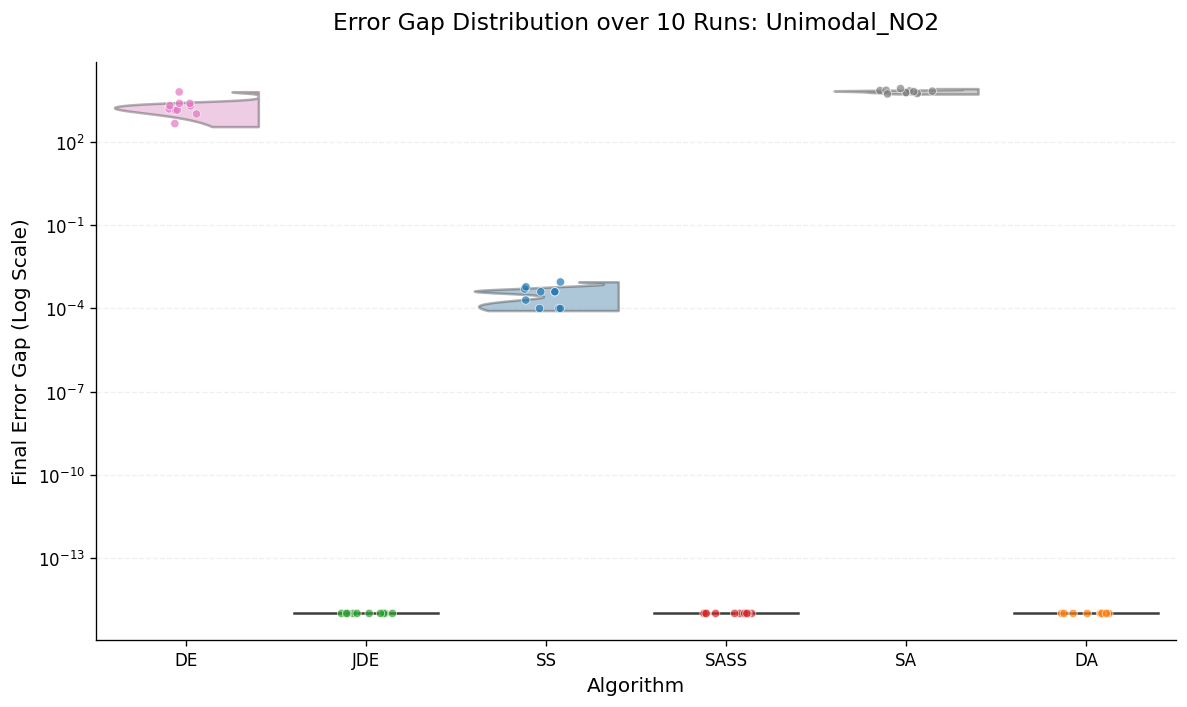
\includegraphics[width=\textwidth]{no2_dist.png}
         \label{fig:image11}
     \end{subfigure}
     \hfill
     \begin{subfigure}{0.49\textwidth}
         \centering
         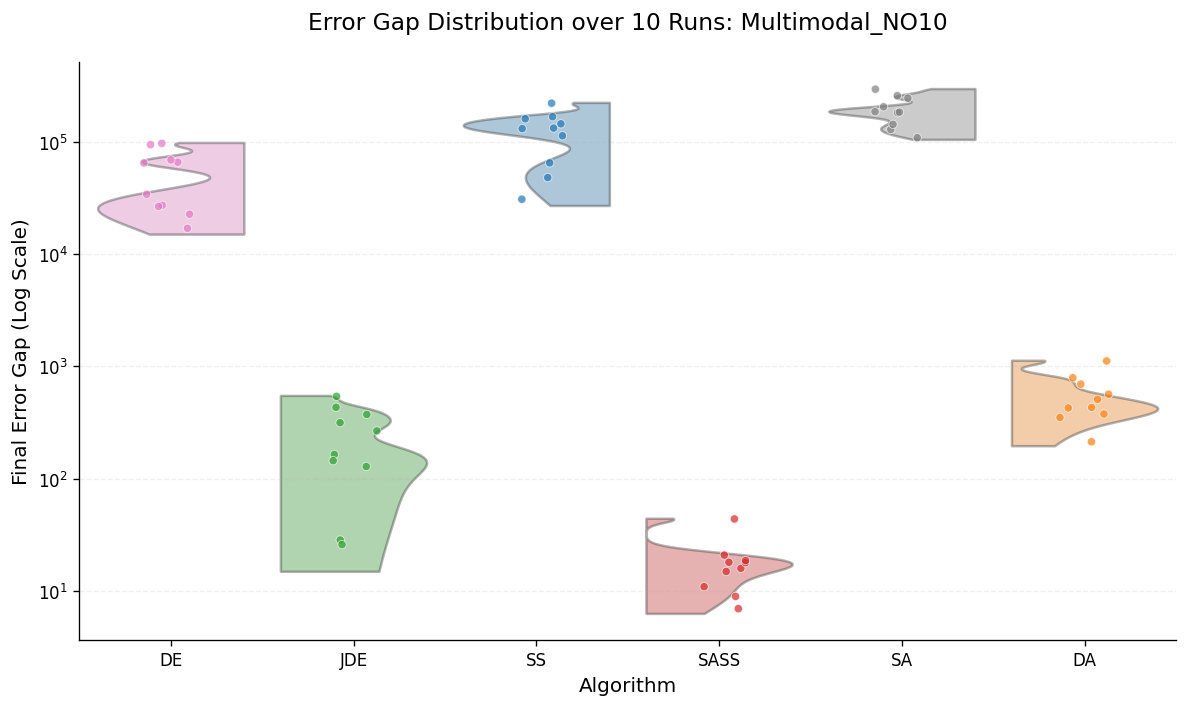
\includegraphics[width=\textwidth]{no10_dist.png}
         \label{fig:image22}
     \end{subfigure}

     \vspace{0.05cm} % Adjust vertical gap between rows

     % Row 2
     \begin{subfigure}{0.49\textwidth}
         \centering
         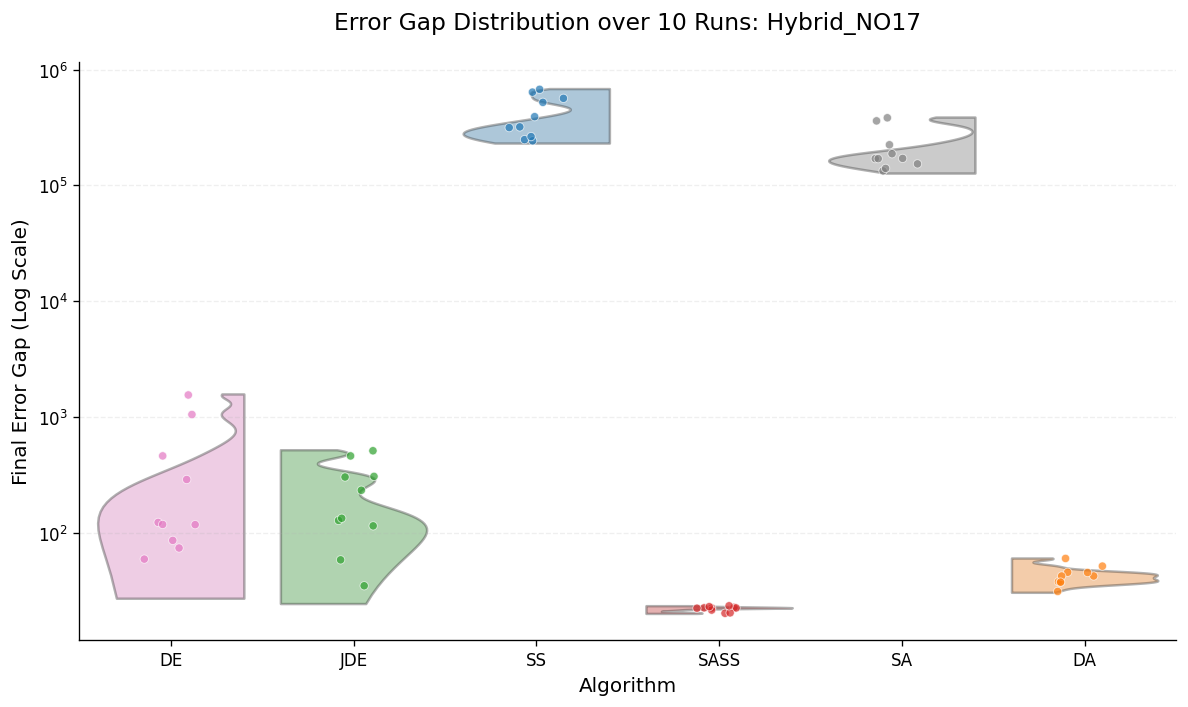
\includegraphics[width=\textwidth]{no17_dist.png}
         \label{fig:image33}
     \end{subfigure}
     \hfill
     \begin{subfigure}{0.49\textwidth}
         \centering
         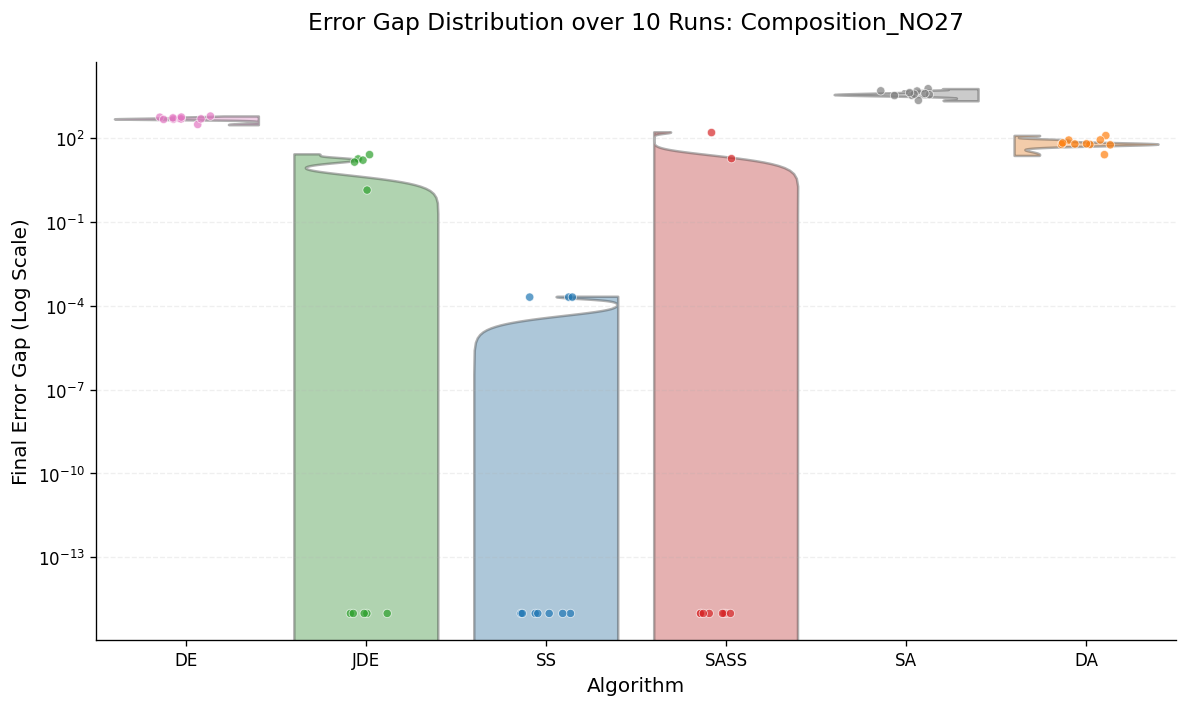
\includegraphics[width=\textwidth]{no27_dist.png}
         \label{fig:image44}
     \end{subfigure}
     
    %  \vspace{0.3cm}
     \caption{Distribution of Final Solutions. Box plots show the distribution of final objective function values across 10 independent runs for each algorithm on each benchmark problem.}
     \label{fig:four_figures_dist}
\end{figure}

From the distribution of final solutions, we can see that the upgraded algorithms (jDE, DA, and SASS) not only achieve better mean values but also show significantly reduced variability compared to their basic counterparts (DE, SA, and SS). However, in the Composition problem (No.27), SS shows a tighter and also better solution distribution than SASS, which is an interesting observation. This could be attributed to the fact that the Composition problem may have a landscape that is more amenable to the search strategy employed by SS, allowing it to consistently find high-quality solutions across multiple runs. In contrast, SASS, while generally effective, may have a more variable performance on this particular problem due to its self-adaptation mechanisms, which can lead to different search trajectories in each run.


\end{document}
